% !TEX root = MusicFormatsMaintainanceGuide.tex

% -------------------------------------------------------------------------
\chapter{MusicFormats distributions}\label{MusicFormats distributions}
% -------------------------------------------------------------------------

%Create a new release
%
%  create a tag with same name
%  describe the release
%  
%  attach the three .zip archives to the release
%  
%  publish the release, il will appear at https://github.com/jacques-menu/musicformats/releases
%  
%  it contains the .zip archives as assets, as well as the source code in .zip and .tar.gz formats
%    
%    
%    
%    git filter-branch --force --index-filter \
%  'git rm -r --cached --ignore-unmatch scripts/musicformats-macos-version-v0.9.65.zip' \
%  --prune-empty --tag-name-filter cat -- --all
%
%ou
%
%git filter-repo --force --index-filter \
%  'git rm -r --cached --ignore-unmatch scripts/musicformats-macos-version-v0.9.65.zip' \
%  --prune-empty --tag-name-filter cat -- --all
%
%puis
%
%git push -f origin master


The \mf\ \repo\ is hosted by \github\ and uses so-called \MainIt{actions} to build the library on \MacOS, \Ubuntu\ and \Windows. The resulting files are then uploaded to the \repo, where they are available to create the distributions for these three \OS s.

The distributions \zip\ archives are supplied with all \mf\ versions, i.e. the current, most recent version of \mf\ (the \default\ \masterBranch\ in the \repo), and the earlier versions such as the \code{v0.9.65} branch.


% -------------------------------------------------------------------------
\section{GitHub actions}
% -------------------------------------------------------------------------

These actions are defined in \code{.yml} files in \directoryName{.github/workflows}:
\begin{lstlisting}[language=Terminal]
jacquesmenu@macmini:~/musicformats-git-dev/.github/workflows > ls -sal
total 24
0 drwxr-xr-x  5 jacquesmenu  staff   160 Aug 24 09:35 .
0 drwxr-xr-x  4 jacquesmenu  staff   128 Aug 22 08:41 ..
8 -rw-r--r--@ 1 jacquesmenu  staff  1366 Aug 23 07:09 build-macos-version.yml
8 -rw-r--r--@ 1 jacquesmenu  staff  1371 Aug 23 07:09 build-ubuntu-version.yml
8 -rw-r--r--@ 1 jacquesmenu  staff  1455 Aug 23 07:08 build-windows-version.yml
\end{lstlisting}

For example, the \Ubuntu\ action in \file{build-ubuntu-version.yml} is shown below. It is executed each time a \code{git push} is performed to the \masterBranch:
\begin{lstlisting}[language=Terminal]
# This is a workflow to build MusicFormats and create a distribution of it

name: Build Ubuntu Version

# Controls when the action will run.
on:
  # Triggers the workflow on push or pull request events but only for the master branch
  push:
    branches: [ master ]
  pull_request:
    branches: [ master ]

  # Allows you to run this workflow manually from the Actions tab
  workflow_dispatch:

# A workflow run is made up of one or more jobs that can run sequentially or in parallel
jobs:
  # This workflow contains a single job called "build"
  build:
    # The type of runner that the job will run on
    runs-on: ubuntu-latest

    # Steps represent a sequence of tasks that will be executed as part of the job
    steps:
      # Checks-out your repository under $GITHUB_WORKSPACE, so your job can access it
      - uses: actions/checkout@v2

      - name: Build MusicFormats for Ubuntu
        run: make -C build

      - name: Upload libraries and executables for Ubuntu
        uses: actions/upload-artifact@v2
        with:
          name: musicformats-ubuntu-version
          path: |
            MusicFormatsVersionNumber.txt
            MusicFormatsVersionDate.txt
            build/bin
            build/lib
            documentation/IntroductionToMusicXML/IntroductionToMusicXML.pdf
            documentation/MusicFormatsUserGuide/MusicFormatsUserGuide.pdf
\end{lstlisting}

After a push to the \masterBranch:
\begin{lstlisting}[language=Terminal]
jacquesmenu@macmini: ~/musicformats-git-dev > git commit -m "Switched from C++11 to C++17 for <filesystem>" -a[master 77d3d29] Switched from C++11 to C++17 for <filesystem>
 7 files changed, 10 insertions(+), 10 deletions(-)

jacquesmenu@macmini: ~/musicformats-git-dev > git push
Enumerating objects: 33, done.
Counting objects: 100% (33/33), done.
Delta compression using up to 8 threads
Compressing objects: 100% (16/16), done.
Writing objects: 100% (17/17), 1.47 KiB | 1.47 MiB/s, done.
Total 17 (delta 14), reused 0 (delta 0), pack-reused 0
remote: Resolving deltas: 100% (14/14), completed with 13 local objects.
To https://github.com/jacques-menu/musicformats.git
   a880063..77d3d29  master -> master
\end{lstlisting}

we get for example:\\
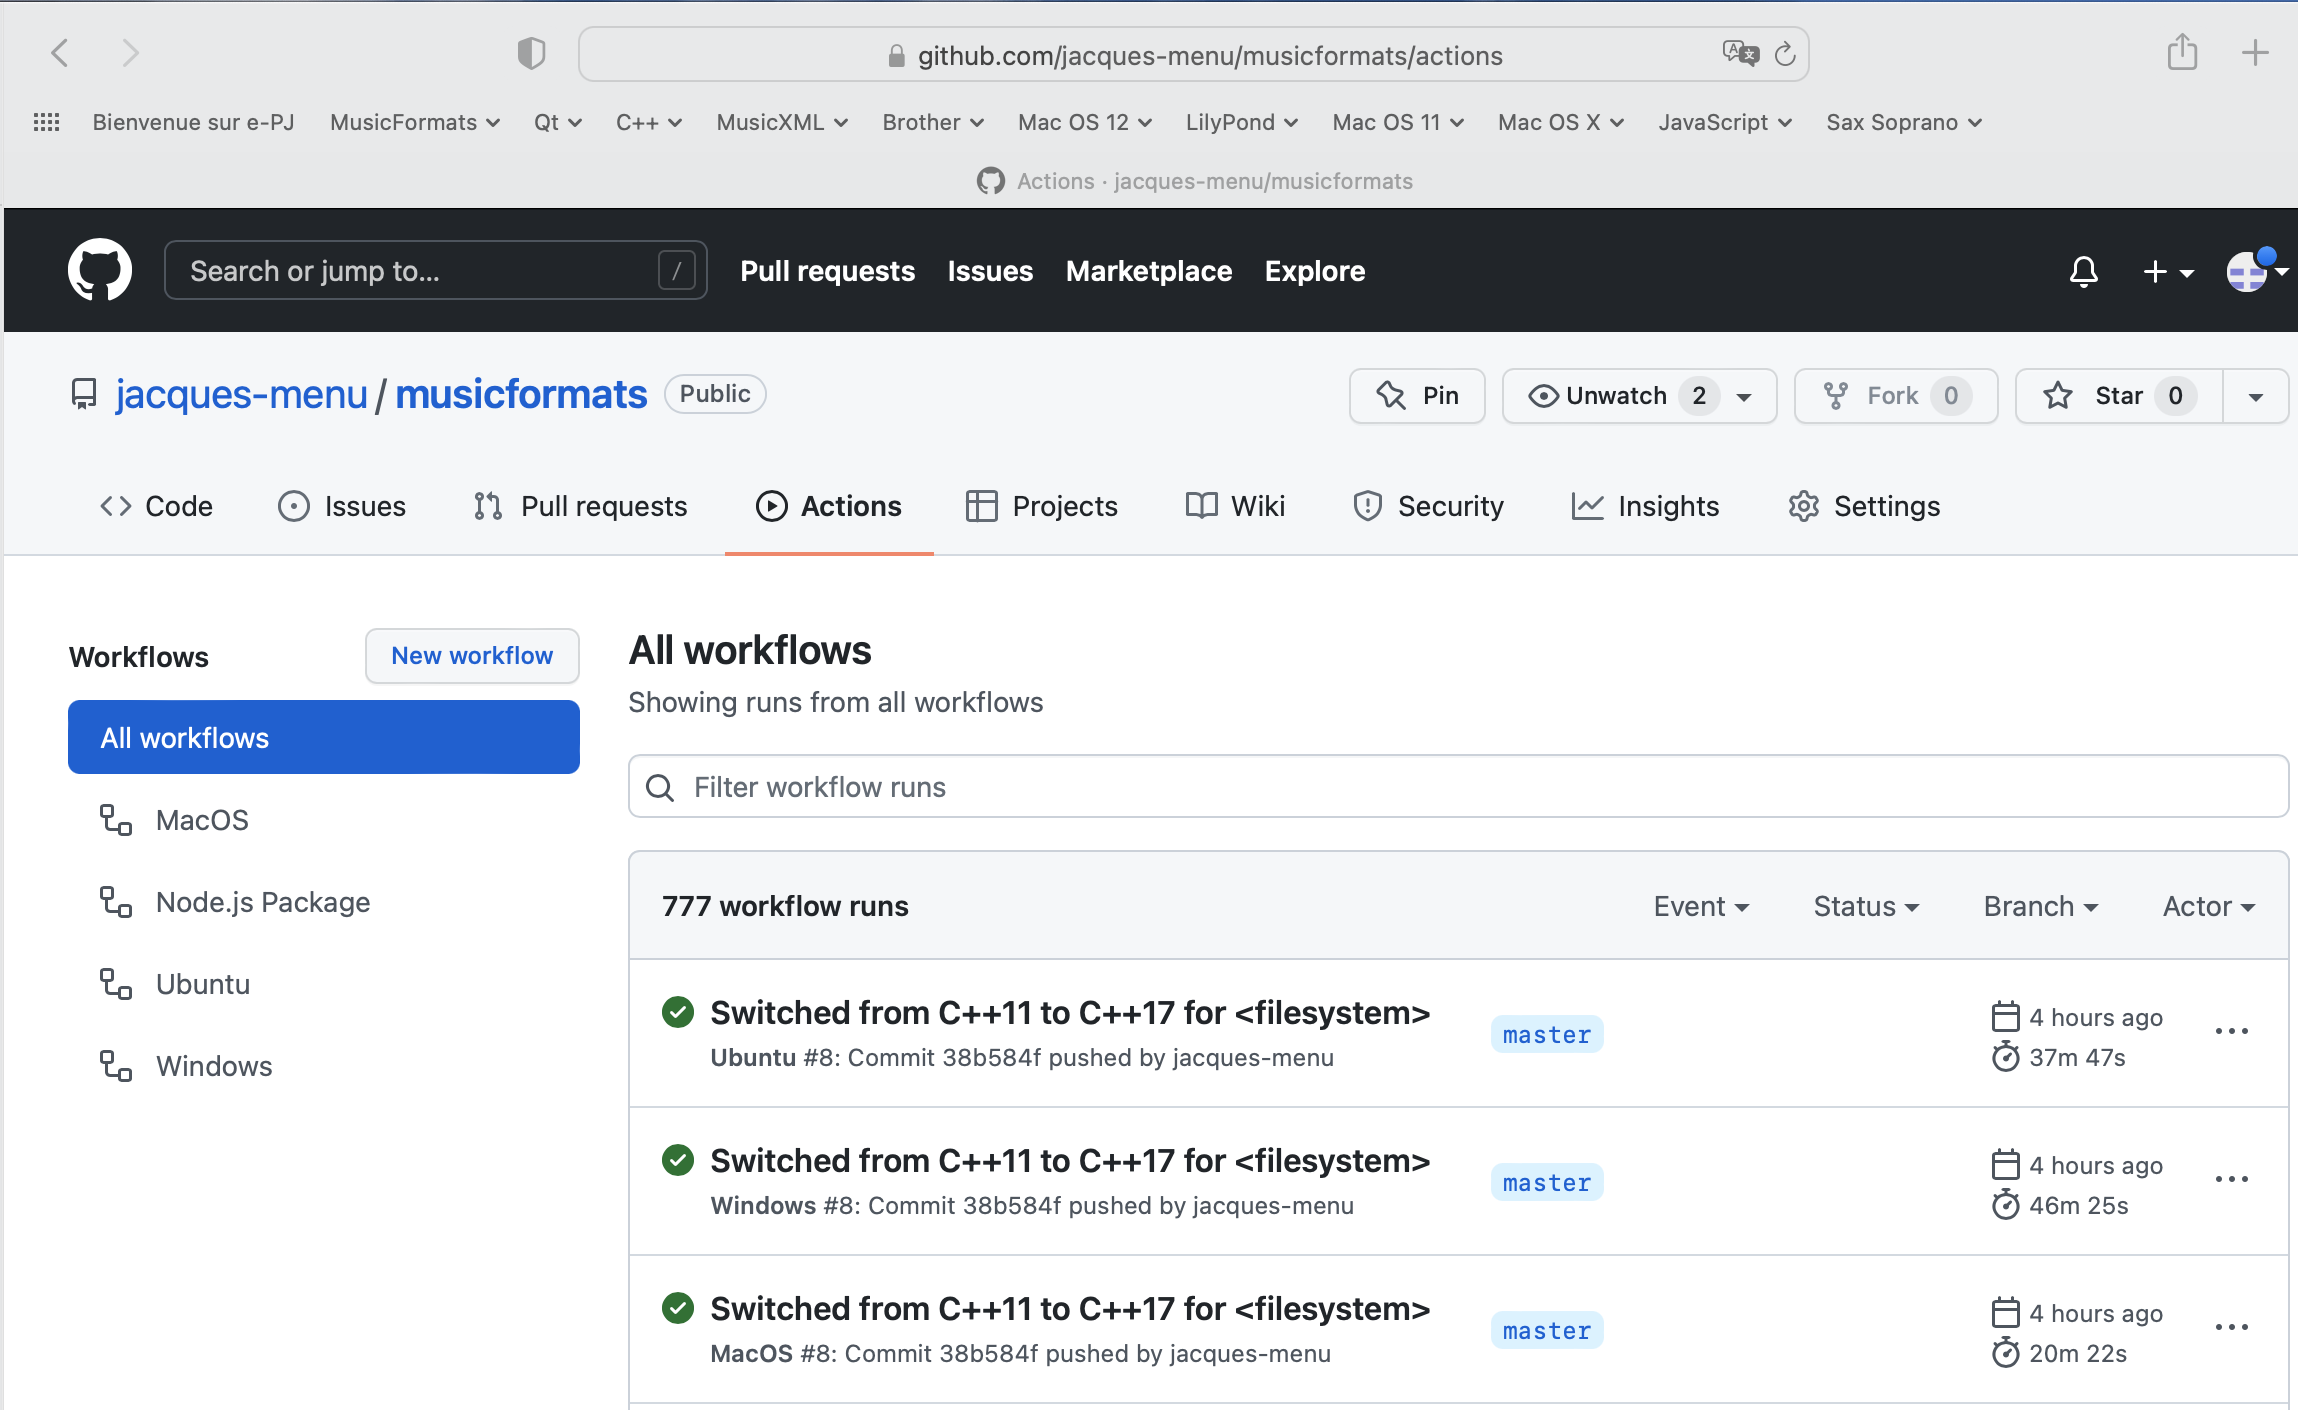
\includegraphics[scale=0.45]{../graphics/GitHubWorkflowsResults.png}

Then cliking on the link leads to:\\
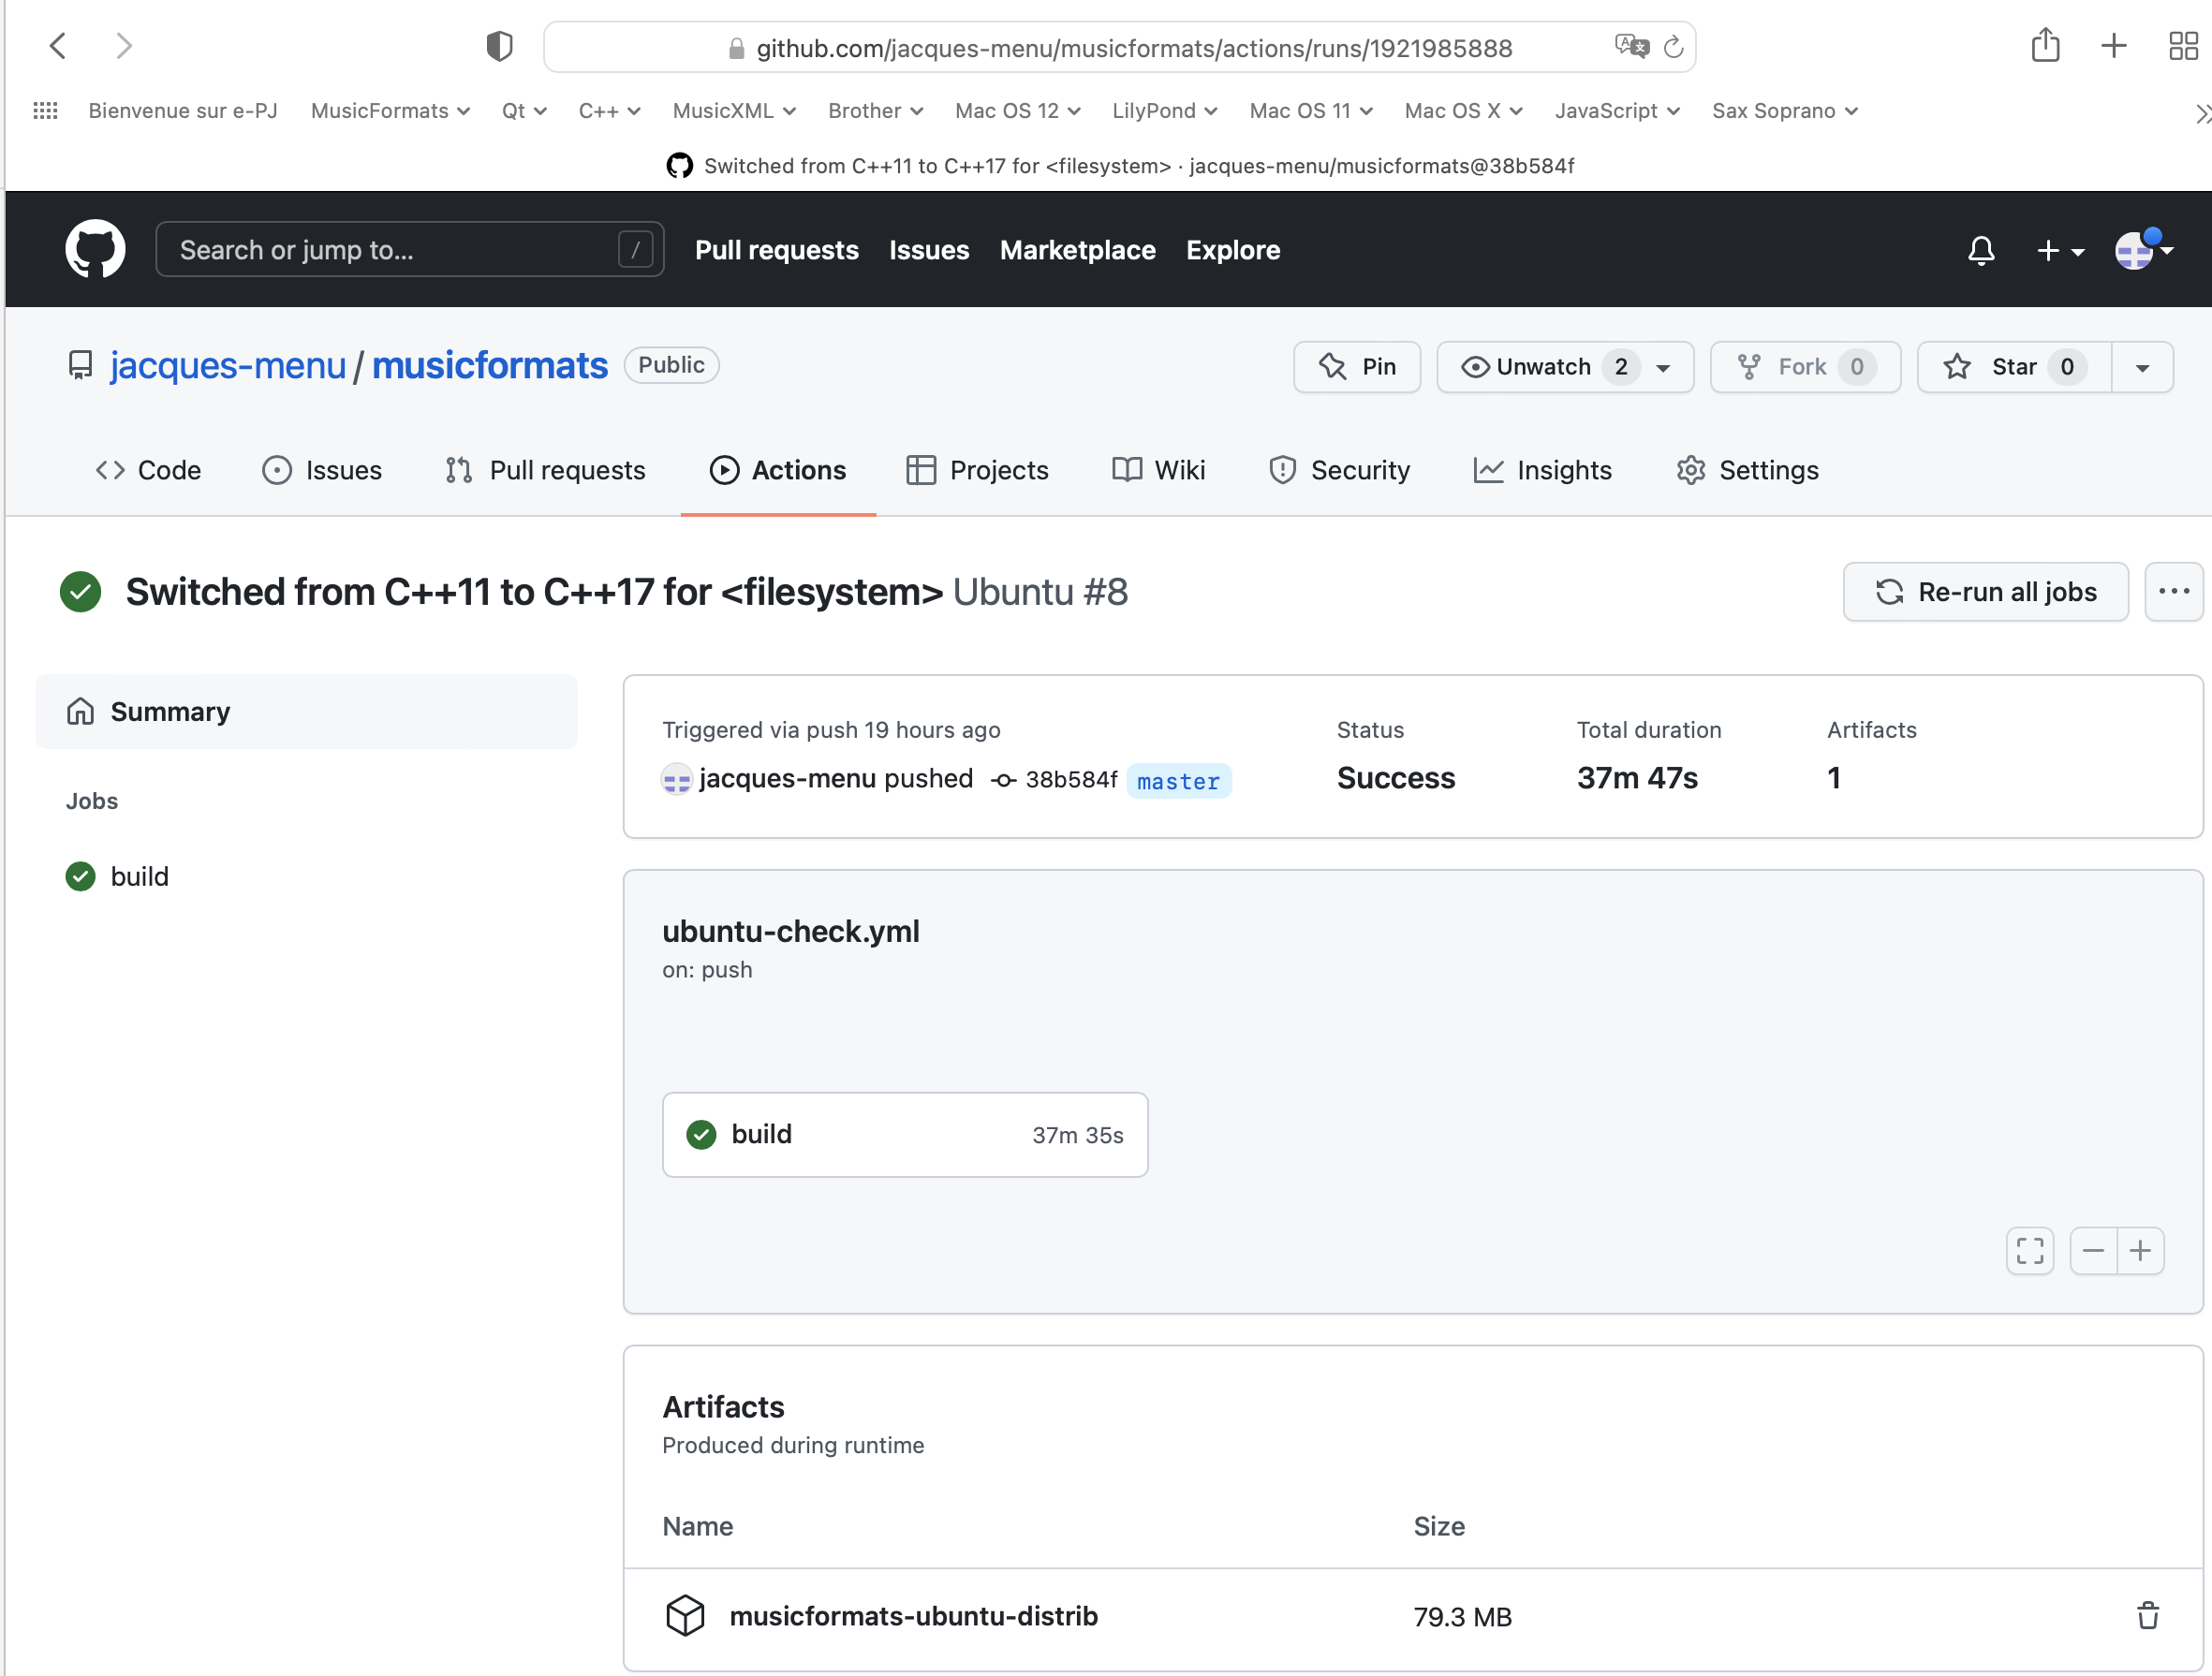
\includegraphics[scale=0.45]{../graphics/GitHubUbuntuActionResult.png}

The \code{musicformats-ubuntu-distrib} archive has to be clicked to get downloaded, since its URL cannot be guessed by an algorithm (it contains numbers internal to \github).

Doing so for the three distributions, we get the following, here in the \directoryName{Downloads} folder on \MacOS, with the \zip\ archives are automatically uncompressed :
\begin{lstlisting}[language=Terminal]
jacquesmenu@macmini: ~/Downloads > ls -sal musicformats-*-distrib
musicformats-macos-distrib:
total 8
0 drwx------@  5 jacquesmenu  staff   160 Mar  3 09:18 .
0 drwx------+ 72 jacquesmenu  staff  2304 Mar  3 09:18 ..
8 -rw-r--r--@  1 jacquesmenu  staff     6 Mar  3 07:10 MusicFormatsVersionNumber.txt
0 drwxr-xr-x@  3 jacquesmenu  staff    96 Mar  3 09:18 build
0 drwxr-xr-x@  4 jacquesmenu  staff   128 Mar  3 09:18 documentation

musicformats-ubuntu-distrib:
total 8
0 drwx------@  5 jacquesmenu  staff   160 Mar  3 09:18 .
0 drwx------+ 72 jacquesmenu  staff  2304 Mar  3 09:18 ..
8 -rw-r--r--@  1 jacquesmenu  staff     6 Mar  3 07:31 MusicFormatsVersionNumber.txt
0 drwxr-xr-x@  4 jacquesmenu  staff   128 Mar  3 09:18 build
0 drwxr-xr-x@  4 jacquesmenu  staff   128 Mar  3 09:18 documentation

musicformats-windows-distrib:
total 8
0 drwx------@  5 jacquesmenu  staff   160 Mar  3 09:18 .
0 drwx------+ 72 jacquesmenu  staff  2304 Mar  3 09:18 ..
8 -rw-r--r--@  1 jacquesmenu  staff     6 Mar  3 07:43 MusicFormatsVersionNumber.txt
0 drwxr-xr-x@  4 jacquesmenu  staff   128 Mar  3 09:18 build
0 drwxr-xr-x@  4 jacquesmenu  staff   128 Mar  3 09:18 documentation
\end{lstlisting}

\begin{lstlisting}[language=Terminal]
jacquesmenu@macmini: ~/Downloads > ls -sal musicformats-ubuntu-distrib/*
8 -rw-r--r--@ 1 jacquesmenu  staff  6 Mar  3 07:31 musicformats-ubuntu-distrib/MusicFormatsVersionNumber.txt

musicformats-ubuntu-distrib/build:
total 0
0 drwxr-xr-x@  4 jacquesmenu  staff  128 Mar  3 09:18 .
0 drwx------@  5 jacquesmenu  staff  160 Mar  3 09:18 ..
0 drwxr-xr-x@ 25 jacquesmenu  staff  800 Mar  3 09:18 bin
0 drwxr-xr-x@  4 jacquesmenu  staff  128 Mar  3 09:18 lib

musicformats-ubuntu-distrib/documentation:
total 0
0 drwxr-xr-x@ 4 jacquesmenu  staff  128 Mar  3 09:18 .
0 drwx------@ 5 jacquesmenu  staff  160 Mar  3 09:18 ..
0 drwxr-xr-x@ 3 jacquesmenu  staff   96 Mar  3 09:18 IntroductionToMusicXML
0 drwxr-xr-x@ 3 jacquesmenu  staff   96 Mar  3 09:18 MusicFormatsUserGuide
\end{lstlisting}

\begin{lstlisting}[language=Terminal]
jacquesmenu@macmini: ~/Downloads > ls -sal musicformats-ubuntu-distrib/*/*
musicformats-ubuntu-distrib/build/bin:
total 2272
  0 drwxr-xr-x@ 25 jacquesmenu  staff     800 Mar  3 09:18 .
  0 drwxr-xr-x@  4 jacquesmenu  staff     128 Mar  3 09:18 ..
 96 -rw-r--r--@  1 jacquesmenu  staff   49008 Mar  3 07:31 LilyPondIssue34
 96 -rw-r--r--@  1 jacquesmenu  staff   49048 Mar  3 07:31 Mikrokosmos3Wandering
 96 -rw-r--r--@  1 jacquesmenu  staff   47280 Mar  3 07:31 MusicAndHarmonies
 96 -rw-r--r--@  1 jacquesmenu  staff   47272 Mar  3 07:31 RandomChords
 96 -rw-r--r--@  1 jacquesmenu  staff   47272 Mar  3 07:31 RandomMusic
 72 -rw-r--r--@  1 jacquesmenu  staff   33848 Mar  3 07:31 countnotes
 40 -rw-r--r--@  1 jacquesmenu  staff   17648 Mar  3 07:31 displayMusicformatsHistory
 40 -rw-r--r--@  1 jacquesmenu  staff   17648 Mar  3 07:31 displayMusicformatsVersion
104 -rw-r--r--@  1 jacquesmenu  staff   50400 Mar  3 07:31 msdlconverter
544 -rw-r--r--@  1 jacquesmenu  staff  276024 Mar  3 07:31 partsummary
 88 -rw-r--r--@  1 jacquesmenu  staff   43768 Mar  3 07:31 readunrolled
 80 -rw-r--r--@  1 jacquesmenu  staff   39064 Mar  3 07:31 xml2brl
 80 -rw-r--r--@  1 jacquesmenu  staff   39104 Mar  3 07:31 xml2gmn
 48 -rw-r--r--@  1 jacquesmenu  staff   23192 Mar  3 07:31 xml2guido
 72 -rw-r--r--@  1 jacquesmenu  staff   34816 Mar  3 07:31 xml2ly
 88 -rw-r--r--@  1 jacquesmenu  staff   42928 Mar  3 07:31 xml2midi
 80 -rw-r--r--@  1 jacquesmenu  staff   39104 Mar  3 07:31 xml2xml
 88 -rw-r--r--@  1 jacquesmenu  staff   43416 Mar  3 07:31 xmlclone
 48 -rw-r--r--@  1 jacquesmenu  staff   22616 Mar  3 07:31 xmlfactory
160 -rw-r--r--@  1 jacquesmenu  staff   79440 Mar  3 07:31 xmliter
 56 -rw-r--r--@  1 jacquesmenu  staff   28472 Mar  3 07:31 xmlread
 64 -rw-r--r--@  1 jacquesmenu  staff   28704 Mar  3 07:31 xmltranspose
 40 -rw-r--r--@  1 jacquesmenu  staff   17360 Mar  3 07:31 xmlversion

musicformats-ubuntu-distrib/build/lib:
total 158600
     0 drwxr-xr-x@ 4 jacquesmenu  staff       128 Mar  3 09:18 .
     0 drwxr-xr-x@ 4 jacquesmenu  staff       128 Mar  3 09:18 ..
113728 -rw-r--r--@ 1 jacquesmenu  staff  58227464 Mar  3 07:31 libmusicformats.a
 44872 -rw-r--r--@ 1 jacquesmenu  staff  22971160 Mar  3 07:31 libmusicformats.so

musicformats-ubuntu-distrib/documentation/IntroductionToMusicXML:
total 1704
   0 drwxr-xr-x@ 3 jacquesmenu  staff      96 Mar  3 09:18 .
   0 drwxr-xr-x@ 4 jacquesmenu  staff     128 Mar  3 09:18 ..
1704 -rw-r--r--@ 1 jacquesmenu  staff  869211 Mar  3 07:31 IntroductionToMusicXML.pdf

musicformats-ubuntu-distrib/documentation/MusicFormatsUserGuide:
total 3000
   0 drwxr-xr-x@ 3 jacquesmenu  staff       96 Mar  3 09:18 .
   0 drwxr-xr-x@ 4 jacquesmenu  staff      128 Mar  3 09:18 ..
3000 -rw-r--r--@ 1 jacquesmenu  staff  1532300 Mar  3 07:31 MusicFormatsUserGuide.pdf
\end{lstlisting}

The contents of \directoryName{musicformats-windows-distrib} differs in the \directoryName{lib} contents:
\begin{lstlisting}[language=Terminal]
jacquesmenu@macmini: ~/Downloads > ls -sal musicformats-windows-distrib/build/lib/
total 37672
    0 drwxr-xr-x@ 4 jacquesmenu  staff       128 Mar  3 09:18 .
    0 drwxr-xr-x@ 4 jacquesmenu  staff       128 Mar  3 09:18 ..
14768 -rw-r--r--@ 1 jacquesmenu  staff   7558913 Mar  3 07:44 musicformats.exp
22904 -rw-r--r--@ 1 jacquesmenu  staff  11726392 Mar  3 07:44 musicformats.lib
\end{lstlisting}

For \MacOS, there is no \directoryName{lib} directory, since the executables in \directoryName{bin} are self-sufficient. They can be placed anywhere on a disk except the trash. Usually, they are placed in the \directoryName{/Applications} directory.

%These distributions are in the form of \zip\ files. They are are available from \url{https://github.com/jacques-menu/musicformats/tree/master/distrib}, as well as the documentation PDF files and version number:
%\begin{lstlisting}[language=Terminal]
%jacquesmenu@macmini: ~/musicformats_local_clone/distrib > ls -sal
%total 150088
%     0 drwxr-xr-x   8 jacquesmenu  staff       256 Feb 16 07:47 .
%     0 drwxr-xr-x  22 jacquesmenu  staff       704 Feb 16 07:47 ..
%  1672 -rw-r--r--   1 jacquesmenu  staff    854294 Feb 16 07:47 IntroductionToMusicXML.pdf
%  1976 -rw-r--r--   1 jacquesmenu  staff   1008702 Feb 16 07:47 MusicFormatsUserGuide.pdf
%108168 -rw-r--r--   1 jacquesmenu  staff  55378423 Feb 16 07:47 MusicFormatsForMacOS.zip
% 34080 -rw-r--r--   1 jacquesmenu  staff  17445663 Feb 16 07:47 MusicFormatsForUbuntu.zip
%  4184 -rw-r--r--   1 jacquesmenu  staff   2139537 Feb 16 07:47 MusicFormatsForWindows.zip
%     8 -rw-r--r--   1 jacquesmenu  staff         6 Feb 16 07:47 MusicFormatsVersionNumber.txt
%\end{lstlisting}


% -------------------------------------------------------------------------
\subsection{Creating the distributions}
% -------------------------------------------------------------------------

The hierarchy in the \directoryName{musicformats-*-distrib} directories comes from the \mf\ \repo\ untouched, which is not convenient for the users.

Their contents is thus re-structured by \scripts{MakeMusicFormatsDistributions.bash}:
\begin{lstlisting}[language=Terminal]
jacquesmenu@macmini: ~/musicformats-git-dev > scripts/MakeMusicFormatsDistributions.bash
... ... ...

==> final distrib contents:
----------------------------------------------

  4208 -rw-r--r--  1 jacquesmenu  staff   2153547 Mar  3 12:55 /Users/jacquesmenu/musicformats-git-dev/distrib/MusicFormatsForWindows.zip
 34576 -rw-r--r--  1 jacquesmenu  staff  17559638 Mar  3 12:55 /Users/jacquesmenu/musicformats-git-dev/distrib/MusicFormatsForUbuntu.zip
109512 -rw-r--r--  1 jacquesmenu  staff  55888914 Mar  3 12:55 /Users/jacquesmenu/musicformats-git-dev/distrib/MusicFormatsForMacOS.zip
  1704 -rw-r--r--@ 1 jacquesmenu  staff    869211 Mar  3 07:10 /Users/jacquesmenu/musicformats-git-dev/distrib/IntroductionToMusicXML.pdf
  3000 -rw-r--r--@ 1 jacquesmenu  staff   1532300 Mar  3 07:10 /Users/jacquesmenu/musicformats-git-dev/distrib/MusicFormatsUserGuide.pdf
     8 -rw-r--r--@ 1 jacquesmenu  staff         6 Mar  3 07:10 /Users/jacquesmenu/musicformats-git-dev/distrib/MusicFormatsVersionNumber.txt

/Users/jacquesmenu/musicformats-git-dev/distrib/MusicFormatsForWindows:
total 8
0 drwxr-xr-x  16 jacquesmenu  staff  512 Mar  3 12:55 ..
0 drwxr-xr-x   5 jacquesmenu  staff  160 Mar  3 12:55 .
0 drwxr-xr-x@  4 jacquesmenu  staff  128 Mar  3 09:18 lib
0 drwxr-xr-x@ 25 jacquesmenu  staff  800 Mar  3 09:18 bin
8 -rw-r--r--@  1 jacquesmenu  staff    6 Mar  3 07:43 MusicFormatsVersionNumber.txt

/Users/jacquesmenu/musicformats-git-dev/distrib/MusicFormatsForUbuntu:
total 8
0 drwxr-xr-x  16 jacquesmenu  staff  512 Mar  3 12:55 ..
0 drwxr-xr-x   5 jacquesmenu  staff  160 Mar  3 12:55 .
0 drwxr-xr-x@  4 jacquesmenu  staff  128 Mar  3 09:18 lib
0 drwxr-xr-x@ 25 jacquesmenu  staff  800 Mar  3 09:18 bin
8 -rw-r--r--@  1 jacquesmenu  staff    6 Mar  3 07:31 MusicFormatsVersionNumber.txt

/Users/jacquesmenu/musicformats-git-dev/distrib/MusicFormatsForMacOS:
total 8
0 drwxr-xr-x  16 jacquesmenu  staff  512 Mar  3 12:55 ..
0 drwxr-xr-x   4 jacquesmenu  staff  128 Mar  3 12:55 .
0 drwxr-xr-x@ 25 jacquesmenu  staff  800 Mar  3 07:10 bin
8 -rw-r--r--@  1 jacquesmenu  staff    6 Mar  3 07:10 MusicFormatsVersionNumber.txt
\end{lstlisting}

The contents of \distrib\ is now:
\begin{lstlisting}[language=Terminal]
jacquesmenu@macmini: ~/musicformats-git-dev/distrib > ls -sal
total 154128
     0 drwxr-xr-x  16 jacquesmenu  staff       512 Mar  3 13:18 .
     0 drwxr-xr-x  35 jacquesmenu  staff      1120 Mar  3 07:13 ..
    24 -rw-r--r--@  1 jacquesmenu  staff      8196 Feb 24 13:33 .DS_Store
  1704 -rw-r--r--@  1 jacquesmenu  staff    869211 Mar  3 07:10 IntroductionToMusicXML.pdf
     0 drwxr-xr-x   4 jacquesmenu  staff       128 Mar  3 13:18 MusicFormatsForMacOS
109960 -rw-r--r--   1 jacquesmenu  staff  55888914 Mar  3 13:18 MusicFormatsForMacOS.zip
     0 drwxr-xr-x   5 jacquesmenu  staff       160 Mar  3 13:18 MusicFormatsForUbuntu
 35216 -rw-r--r--   1 jacquesmenu  staff  17559638 Mar  3 13:18 MusicFormatsForUbuntu.zip
     0 drwxr-xr-x   5 jacquesmenu  staff       160 Mar  3 13:18 MusicFormatsForWindows
  4208 -rw-r--r--   1 jacquesmenu  staff   2153547 Mar  3 13:18 MusicFormatsForWindows.zip
  3000 -rw-r--r--@  1 jacquesmenu  staff   1532300 Mar  3 07:10 MusicFormatsUserGuide.pdf
     8 -rw-r--r--@  1 jacquesmenu  staff         6 Mar  3 07:10 MusicFormatsVersionNumber.txt
     8 -rwxr-xr-x@  1 jacquesmenu  staff        95 Mar  3 12:54 doClean.bash
     0 drwx------@  6 jacquesmenu  staff       192 Mar  3 10:56 musicformats-macos-distrib
     0 drwx------@  6 jacquesmenu  staff       192 Mar  3 10:56 musicformats-ubuntu-distrib
     0 drwx------@  6 jacquesmenu  staff       192 Mar  3 10:56 musicformats-windows-distrib
\end{lstlisting}


% -------------------------------------------------------------------------
\subsection{Security issue in recent MacOS\texttrademark\ versions}
% -------------------------------------------------------------------------

\MacOS\ gets more and more stringent over time regarding security. The \OS\ part in charge of this is named \Gatekeeper.

When downloading the \mf\ distributions from the \repo\ on versions up to 10 (\Main{High Sierra}), the executables in \code{bin} are usable alright.

From version 11 (\Main{Catalina}) on, though, the executables you get are not executable actually, because their developer is unknown to the \OS, and actions have to be taken for them to be usable.

The trouble is that these executables are in {\it \quarantine} by default. To make them usable, they have to quit quarantine and explicitly be made executable.

This is done this way using \code{chmod} and \code{xattr} in \scripts{MakeMusicFormatsDistributions.bash}:
\begin{lstlisting}[language=Terminal]
  # make the executables actually executable
  chmod +x bin/*
  xattr -d com.apple.quarantine bin/*
\end{lstlisting}
%codesign --sign - --force --deep %%%JMI not necessary

%%%JMI see user doc???

From then on, the \mf\ executables can be used seamlessly on the given machine.

Having to perform the preceding task for each executable is the price to pay for security. And it has to be perfomed again when installing new versions\dots

The above can be done in the \GUI\ file by file too. Right after you got the message above:
\begin{itemize}
\item  open \MainIt{System Preferences}, choose the \MainIt{Security \& Privacy} tab, and there click on the \MainIt{General button};

\item click on the lock at the bottom left of the dialog to make changes:\\
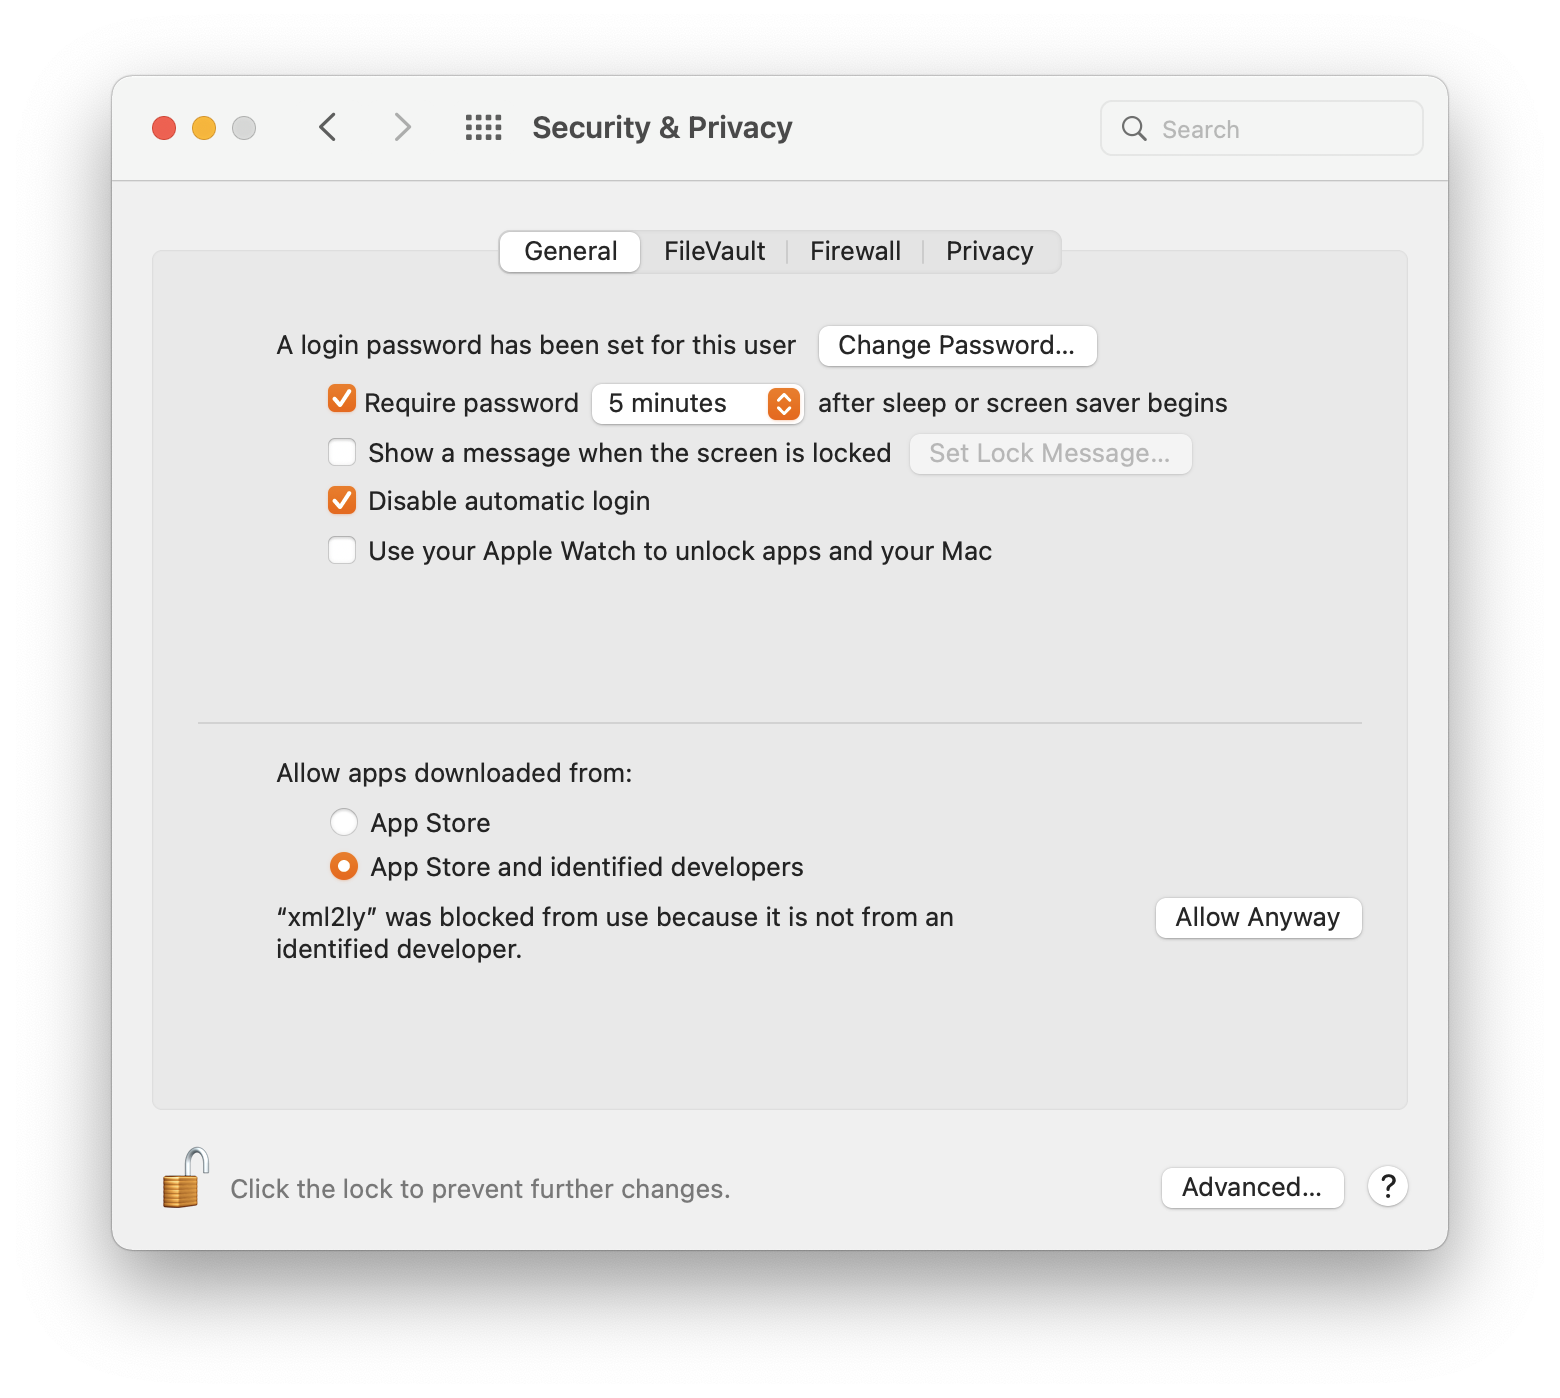
\includegraphics[scale=0.35]{../graphics/MacOSAllowAnyway.png}

\item click on the \MainIt{Allow Anyway} button.
%%%JMI sudo spctl --master-disable to create a Anywhere radio button
%jacquesmenu@macmini > spctl --status
%assessments enabled

\end{itemize}

Re-execute the executable from the command line. This pops-up a dialog to confirm you actually want to use this software:\\
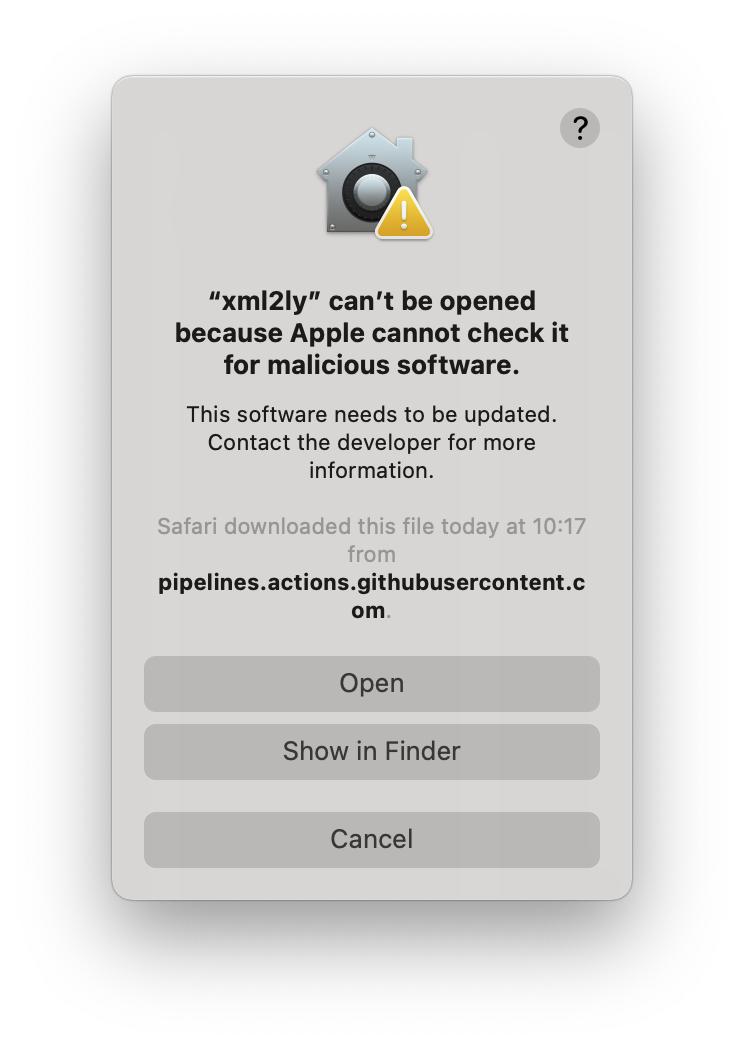
\includegraphics[scale=0.35]{../graphics/MacOSConfirmOpening.png}

Click on the \MainIt{Open} button to register the executable in \Gatekeeper\ and go ahead.
